\documentclass[11pt]{article}

\usepackage[letterpaper,margin=1in]{geometry}
\usepackage[T1]{fontenc}
\usepackage{lmodern}
\usepackage{microtype}
\usepackage{amsmath,amssymb,amsthm,mathtools}
\usepackage{booktabs,tabularx,longtable,array}
\usepackage{graphicx}
\usepackage[dvipsnames]{xcolor}
\usepackage{enumitem}
\usepackage[round,authoryear]{natbib}
\usepackage{xurl}
\usepackage{fancyhdr}
\usepackage{hyperref}
\usepackage[nameinlink,noabbrev]{cleveref}

\definecolor{Ink}{HTML}{17324D}
\definecolor{Accent}{HTML}{B43C4E}
\definecolor{Gold}{HTML}{9A6A12}
\definecolor{Green}{HTML}{176B5B}
\hypersetup{
  colorlinks=true,
  linkcolor=Ink,
  citecolor=Ink,
  urlcolor=Accent,
  pdftitle={The Dottie Parabolic Fold and the Marked Spire of Reciprocal Tetration},
  pdfauthor={Nick},
  pdfsubject={Parabolic dynamics, antiholomorphic half-step, horn maps, and certified reciprocal-tetration dynamics}
}

\pagestyle{fancy}
\fancyhf{}
\fancyhead[L]{\small The Dottie parabolic fold and marked spire}
\fancyhead[R]{\small Nick}
\fancyfoot[C]{\thepage}
\setlength{\headheight}{14pt}

\newtheorem{theorem}{Theorem}[section]
\newtheorem{proposition}[theorem]{Proposition}
\newtheorem{corollary}[theorem]{Corollary}
\newtheorem{lemma}[theorem]{Lemma}
\theoremstyle{definition}
\newtheorem{definition}[theorem]{Definition}
\newtheorem{certificate}[theorem]{Directed certificate}
\newtheorem{observation}[theorem]{Measured observation}
\theoremstyle{remark}
\newtheorem{remark}[theorem]{Remark}

\newcommand{\C}{\mathbb C}
\newcommand{\R}{\mathbb R}
\newcommand{\e}{\mathrm e}
\newcommand{\expmone}{\operatorname{expm1}}
\newcommand{\Logp}{\operatorname{Log}}
\newcommand{\status}[1]{\textsf{\textbf{#1}}}
\newcommand{\abs}[1]{\lvert#1\rvert}
\newcommand{\norm}[1]{\lVert#1\rVert}

\title{\bfseries The Dottie Parabolic Fold and the Marked Spire\\[0.35em]
\large Cylinder--horn equations, directed local dynamics, and conditional rail asymptotics}
\author{Nick\\\small Independent Researcher}
\date{Research preprint v1.0 -- August 12, 2026}

\begin{document}
\maketitle

\begin{abstract}
On the invariant imaginary-parameter slice of reciprocal tetration, the two-step scalar map is
\[
  g_{iy}(z)=\exp\!\bigl(iy\exp(-iyz)\bigr).
\]
Its centerline fixed points admit the exact curve
\[
  Y(u)=u\sec u\,\e^{-u\tan u},\qquad
  Z(u)=\e^{u\tan u+iu},
\]
and the multiplier is $(u\sec u)^2$.  Hence the parabolic fold occurs precisely at the Dottie number $d=\cos d$, with
\[
  L_*=i\e^{-\sin d},\qquad Z_*=\e^{\sin d+id}.
\]
Baker and Rippon's alternating-conjugate theorem already contains this reciprocal centerline return, its boundary location and multiplier bookkeeping, and the antiholomorphic half-step whose square is the return \citep[Theorem~8.1 and the remark on p.~200]{BakerRippon1989Composite}.  Their decimal constants on p.~189 are exactly $\pi/2-d$ and $Z_*$, although the Dottie identification is not made there.  Our contribution begins with that exact identification and continues through the quadratic fold, the Dottie-normalized simple parabolic germ, and the physical return structure.  More generally, the autonomous one-base return and reciprocal return are the $c=1$ and $c=-1$ slices of the same two-base family $E_\kappa\circ E_{\kappa+\delta}$, $c=\e^\delta$.  The two local fixed-point branches yield a sign-adjusted canonical parameter $E$ and formal invariant $b$,
\[
  E=-\bigl(\Lambda_+^{-1}-\Lambda_-^{-1}\bigr)^{-2},\qquad
  b=\Lambda_+^{-1}+\Lambda_-^{-1}.
\]
On a selected Fatou-cylinder continuation, the return is encoded by one horn displacement $S$: $H(\xi)=\xi\exp(2\pi iS(\xi))$.  This gives exact even and odd physical return equations, the odd critical-locus identity $\det_{\R}D_W\delta_o=4(|m|^2-1)$, and explicit Morse equations.  Directed Krawczyk/ball-arithmetic computations isolate principal and additional physical-even minima, a physical-odd minimum, three cap-captured windows of paired periods $639,640,641$, and separate attracting and repelling period-$640$ witnesses.  High-precision parabolic-interpolation estimates of finite multiplier minima through paired period $4800$ approach the additional horn-root box with a measured $p^{-2}$ trend.  A theorem is proved conditional on the still-missing finite-to-horn matching: any selected finite rail satisfying the matching hypotheses obeys
\[
  y_p-y_*=\frac{C_*}{(p-\delta_0)^2}+\frac{A_4}{(p-\delta_0)^4}+O(p^{-5}),
\]
with $C_*$ and $A_4$ explicit in $d$.  The local certificates, finite-parameter bridge, and remaining global continuation problem are kept logically separate.
\end{abstract}

\noindent\textbf{Keywords.} parabolic fixed point; Fatou coordinate; horn map; antiholomorphic dynamics; tetration; interval arithmetic.\\
\textbf{MSC 2020.} 37F10, 37F46, 30D05, 65G30.

\medskip
\noindent\fcolorbox{Ink}{Ink!4}{\parbox{0.955\linewidth}{\small
\textbf{Evidence convention.} \status{Exact} means a consequence of the displayed definitions or a cited theorem.  \status{Certified} means a directed, outward-rounded enclosure tied to a retained replayable record.  \status{Measured} means arbitrary-precision point evidence or a finite raster.  \status{Conditional} states all required hypotheses.  \status{Open} marks a question for which no conclusion is claimed.}}

\section{Setting, clocks, and scope}

The companion foundations paper \citep{NickFoundations2026} studies the reciprocal cyclic-exponential pair
\begin{equation}
  F_L(P,M)=\bigl(\e^{LM},\e^{-LP}\bigr),
  \label{eq:pairmap}
\end{equation}
which is a one-parameter specialization of classical cyclic exponentiation \citep{BakerRippon1989,BakerRippon1989Composite}.  Two pair steps decouple:
\begin{equation}
  F_L^2(P,M)=\bigl(g_L(P),g_{-L}(M)\bigr),
  \qquad
  g_L(z)=\exp\!\bigl(L\exp(-Lz)\bigr).
  \label{eq:scalar}
\end{equation}
On the centerline $L=iy$, the diagonal real form $M=\bar P$ is invariant and a single pair step becomes
\begin{equation}
  H_y(z)=\exp(iy\bar z),
  \qquad H_y^2=g_{iy}.
  \label{eq:halfstep-original}
\end{equation}

This half-step is already the map $g_a(z)=\exp(a\bar z)$ in the remark added in proof by \citet[p.~200]{BakerRippon1989Composite}, specialized to $a=iy$.  To compare it with the additive exponential family, let the second visible base be $b=a^c$.  If $L=\e^\kappa$, $c=\e^\delta$, and
\[
  g_{L,c}(z)=\exp\!\bigl(L\exp(cLz)\bigr),
  \qquad C_{\kappa,c}(z)=\kappa+cLz,
\]
then
\begin{equation}
  C_{\kappa,c}\circ g_{L,c}\circ C_{\kappa,c}^{-1}
  =E_\kappa\circ E_{\kappa+\delta}.
  \label{eq:exponential-slice-completion}
\end{equation}
The equal-base return is the $c=1$ slice $E_\kappa^2$; the reciprocal return is the $c=-1$ slice $E_\kappa\circ E_{\kappa+\pi i}$.  They are sibling slices of this common two-base family, rather than one being a slice of the other.  The family of \citet{RempeSchleicher2008} supplies the standard $E_\kappa$ coordinate setting; \citet{BakerRippon1989Composite} supplies the alternating-conjugate $|c|=1$ setting and, on $L=iy$, exactly the reciprocal value $c=\bar L/L=-1$.  The retained ordered pair, cap marking, and later parity-sensitive return equations are the additional data used here.

We distinguish three clocks.  The symbol $p$ denotes a paired period of $F_{iy}$, $p_{\rm sc}=p/\gcd(p,2)$ the associated period of the holomorphic two-step map $g_{iy}$, and $N$ a local passage/deck count in a Fatou chart.  For $E>0$ on the selected centerline sheet, define the canonical paired phase
\begin{equation}
  \delta=p-\frac{2\pi}{\sqrt E},
  \label{eq:delta-clock}
\end{equation}
using the positive centerline square root.  Along sequences $E_n\to0^+$ and $p_n\to\infty$ for which $p_n-2\pi/\sqrt{E_n}$ remains bounded (and, when needed, converges), $\delta$ denotes the corresponding limiting Lavaurs phase in the physical equations below.  Thus an even paired period $p$ has $p_{\rm sc}=p/2$, while an odd paired period has $p_{\rm sc}=p$.  The integer $N=25$ appearing in the present certificates is a selected access word, not an intrinsic modulus.

Throughout, $\Logp z$ denotes the principal logarithm with $\arg z\in(-\pi,\pi]$.  A subscript $+$ or $-$ denotes the retained upper or lower continuation side at a cut; this continuation side is part of the proof data.

Following \citet{Kaplan2007}, we call the positive solution $d=0.7390851332\ldots$ of $d=\cos d$ the Dottie number.  Baker and Rippon already supply the reciprocal centerline parameter, fixed-point multiplier, and half-step; the contribution here starts by identifying their decimal boundary data exactly with $d$ and then develops the Dottie-centered normalization, fold coefficients, physical return equations, and directed proof objects.  Parabolic analytic classification is due to Écalle and Voronin \citep{Ecalle1985,Voronin1981}; resurgence of Fatou coordinates and horn invariants is developed by \citet{DudkoSauzin2014,DudkoSauzin2015}.  The relevant antiholomorphic classification is given by \citet{GodinRousseau2022}, and generic unfoldings by \citet{MardesicRoussarieRousseau2004,ChristopherRousseau2014,GodinRousseau2023,Rousseau2026}.  No new general classification theorem is claimed.

\section{The exact fixed curve and Dottie fold}

For $0<u<\pi/2$, define
\begin{equation}
  Y(u)=u\sec u\,\e^{-u\tan u},\qquad
  Z(u)=\e^{u\tan u+iu},\qquad
  L(u)=iY(u).
  \label{eq:fixedcurve}
\end{equation}

\begin{theorem}[Exact centerline fixed curve]\label{thm:fixedcurve}
For every $u\in(0,\pi/2)$,
\begin{equation}
  g_{L(u)}(Z(u))=Z(u),
  \qquad
  g_{L(u)}'(Z(u))=(u\sec u)^2.
  \label{eq:fixed-multiplier}
\end{equation}
Moreover,
\begin{equation}
  \frac{Y'(u)}{Y(u)}=\frac1u-u\sec^2u,
  \label{eq:ylogderivative}
\end{equation}
so the following are equivalent on this interval:
\begin{equation}
  Y'(u)=0,
  \qquad u=\cos u,
  \qquad g_{L(u)}'(Z(u))=1.
  \label{eq:dottie-equivalence}
\end{equation}
\end{theorem}

\begin{proof}
The product $Y(u)Z(u)=u\sec u\,\e^{iu}=u+iu\tan u$ gives
\[
  \e^{-L(u)Z(u)}=\e^{u\tan u-iu}.
\]
Multiplication by $L(u)=iY(u)$ and exponentiation yield $Z(u)$.  Since
$g_L'(z)=-L^2\e^{-Lz}g_L(z)$, substitution gives $(u\sec u)^2$.  Logarithmic differentiation of $Y$ gives \cref{eq:ylogderivative}; multiplying its vanishing equation by $u\cos^2u$ yields $\cos^2u=u^2$, hence $u=\cos u$ on the chosen interval.
\end{proof}

The curve and multiplier in \cref{thm:fixedcurve} are the imaginary-axis specialization of Baker--Rippon's fixed-point bookkeeping.  Set
\[
  \sigma(u)=u\tan u+iu,
  \qquad \tau(u)=\overline{\sigma(u)}.
\]
Then
\[
  L(u)=\sigma(u)\e^{-\tau(u)},
  \qquad Z(u)=\e^{\sigma(u)},
  \qquad \sigma(u)\tau(u)=(u\sec u)^2,
\]
which is their parametrization $a=s\e^{-t}$ with multiplier $st$ and $t=\bar s$ \citep[eqs.~(12)--(13), pp.~195--196]{BakerRippon1989Composite}.  At $u=d$, $\sigma(d)=\sin d+id$ has unit modulus, so $L_*$ is precisely the positive-imaginary boundary point of their set $\mathcal C=\{t\e^{-\bar t}:|t|\le1\}$, reported near $0.51i$.  The location, curve, and multiplier are therefore prior results; the equivalence of their boundary coordinate with the named Dottie identity is the next step.

Put
\begin{equation}
  d=\cos d,\qquad s=\sin d,\qquad
  y_*=\e^{-s},\qquad L_*=iy_*,
  \qquad Z_*=\e^{s+id}.
  \label{eq:dottie-data}
\end{equation}

Equation~(8) of \citet[p.~189]{BakerRippon1989Composite} prints
\[
  \theta=0.831711193\ldots,
  \qquad \alpha+i\beta
  =1.449574211\ldots+1.321161232\ldots i.
\]
These are exactly
\[
  \theta=\frac\pi2-d,
  \qquad \alpha+i\beta=\e^{\sin d+id}=Z_*.
\]
Thus their decimals already locate the same parabolic fixed point; the exact Dottie interpretation and fold identity are what are supplied here.

\begin{proposition}[Quadratic fold]\label{prop:quadratic-fold}
As $h\to0$,
\begin{equation}
  Y(d+h)=y_*
  -\frac{y_*(1+s)}{d^2}h^2
  -\frac{2y_*s(1+s)}{3d^3}h^3+O(h^4).
  \label{eq:fold-expansion}
\end{equation}
In particular, the centerline fixed curve has a nondegenerate quadratic fold at $(L_*,Z_*)$.
\end{proposition}

\begin{proof}
Differentiate \cref{eq:ylogderivative} twice, use $d=\cos d$ and $s=\sin d$, and substitute into Taylor's formula.  The quadratic coefficient is nonzero because $y_*,1+s,d>0$.
\end{proof}

\begin{figure}[t]
  \centering
  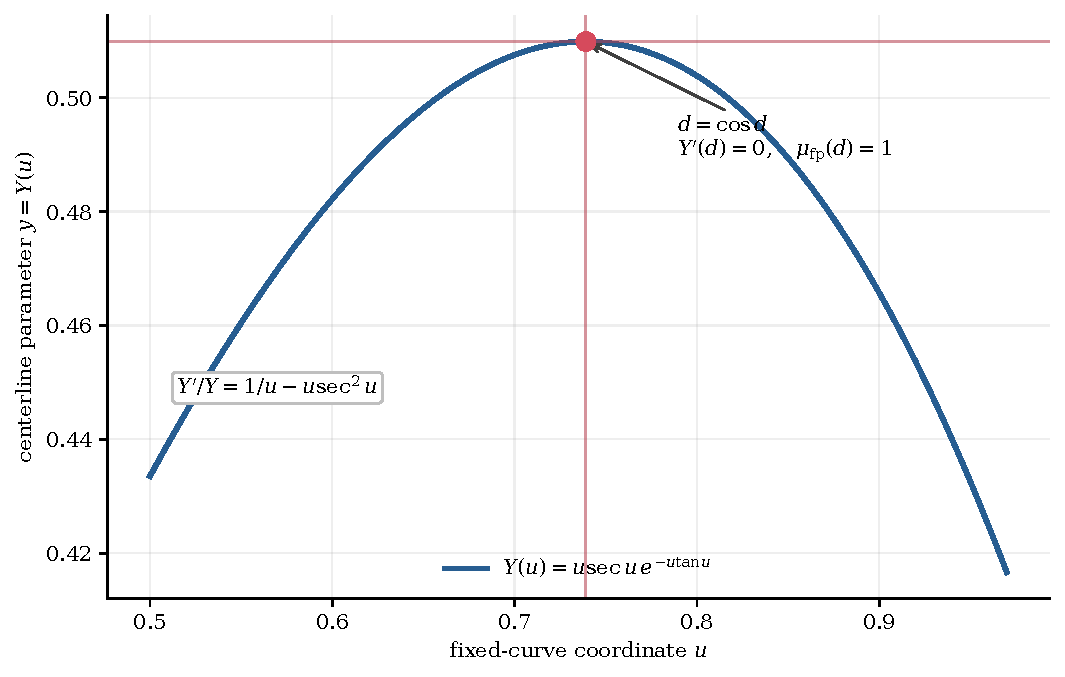
\includegraphics[width=0.96\textwidth]{figures/exact_dottie_fold.pdf}
  \caption{The exact fixed curve.  The multiplier reaches $1$ at the same $u=d$ at which $Y$ folds.  The local parameter displacement is quadratic in $u-d$, the elementary source of the $p^{-2}$ scale.}
  \label{fig:dottie-fold}
\end{figure}

The fold supplies a family-specific realization of the saddle-node/parabolic transit scale; compare the general scaling discussion of \citet{Kuehn2009}.  It does not, by itself, identify a cap-marked finite orbit with a local horn branch.

\section{Normalized germ and antiholomorphic square root}

Let
\begin{equation}
  \alpha=s+id,\qquad
  \rho=\frac{s}{3(1+s)},\qquad
  c_2=\frac{(1+\alpha)(-iy_*)}{2},
  \qquad x=c_2(z-Z_*).
  \label{eq:normalization-data}
\end{equation}
Because $s^2+d^2=1$, $|\alpha|=1$.

\begin{proposition}[Exact normalized germ]\label{prop:germ}
The coordinate in \cref{eq:normalization-data} conjugates the germ of $g_{L_*}$ at $Z_*$ to
\begin{equation}
  f(x)=\frac{1+\alpha}{2\alpha}
  \expmone\!\left(
    \alpha\,\expmone\!\left(\frac{2x}{1+\alpha}\right)
  \right)
  =x+x^2+(1-\rho)x^3+O(x^4).
  \label{eq:normalized-germ}
\end{equation}
The antiholomorphic germ
\begin{equation}
  K(x)=\frac{\expmone(\varkappa\bar x)}{\varkappa},
  \qquad
  \varkappa=\frac{2\alpha}{1+\alpha}
  =1+i\frac{d}{1+s},
  \label{eq:normalized-halfstep}
\end{equation}
satisfies $K^2=f$ exactly.
\end{proposition}

\begin{proof}
Substitute $z=Z_*+x/c_2$ into \cref{eq:scalar}, use $iy_*Z_*=-s+id$, and simplify the two nested exponentials.  The displayed Taylor coefficients follow from the power series of $\expmone$.  Substitution of \cref{eq:normalized-halfstep} into itself, using $\bar\alpha=\alpha^{-1}$ and $\Re\varkappa=1$, gives \cref{eq:normalized-germ}.
\end{proof}

Earlier computations used the half-step scale $\kappa_H=y_*\sqrt\alpha$.  It is compatible with \cref{eq:normalized-halfstep}, but it is not the same constant.  If $\alpha=\e^{i\theta}$, then
\[
  \varkappa=\frac{\sqrt\alpha}{\cos(\theta/2)},
  \qquad
  \frac{\kappa_H}{\varkappa}
  =y_*\cos(\theta/2)=y_*\sqrt{\frac{1+s}{2}}\in\R_{>0}.
\]
The real rescaling $x_{\rm new}=(\kappa_H/\varkappa)x_{\rm old}$ conjugates the two normalizations.

Choose compatible Fatou branches with
\begin{equation}
  \Phi_\sigma(x)=-\frac1x+\rho\log_\sigma x+o(1),
  \label{eq:fatou-asymptotic}
\end{equation}
where $\log_\sigma$ is obtained by the stated upper or lower continuation on the specified petal.  With these compatible normalizations, the half-step has the cylinder lift
\begin{equation}
  \widehat K(W)=\bar W+\frac{\varkappa}{2},
  \qquad \widehat K^2(W)=W+1.
  \label{eq:fatou-halfstep}
\end{equation}
The unnormalized centerline half-step $H_y$ is already present in \citet{BakerRippon1989Composite}.  The contribution of \cref{prop:germ,eq:fatou-halfstep} is its exact Dottie centering and scaling, the normalized germ $K^2=f$, and the compatible Fatou-cylinder lift used by the physical even/odd equations.  This realization lies within the antiholomorphic classification and root structure of \citet{GodinRousseau2022}; the general structure is not new.

The formal Fatou coefficients of \cref{eq:normalized-germ} lie in $\mathbb Q(\alpha)$.  This does not imply that the analytic horn invariants do.  Likewise, the $2\pi i\mathbb Z$ resurgent framework of \citet{DudkoSauzin2014,DudkoSauzin2015} is relevant context, but does not by itself prove an actual Borel singularity at modulus $2\pi$ or nonconvergence for this particular normalization.

\section{Sign-adjusted canonical unfolding variables}

For $y$ near $y_*$, let $u_+(y)$ and $u_-(y)$ be the two local inverse branches of $Y(u)=y$ selected by continuation from the Dottie fold, and set
\begin{equation}
  \Lambda_\pm(y)=2\Logp\!\bigl(u_\pm(y)\sec u_\pm(y)\bigr).
  \label{eq:lambda-branches}
\end{equation}
The quantities $\Lambda_\pm$ use the principal logarithm near $1$, so $\Lambda_\pm\to0$ at the fold.  The inverse-branch labels and square-root choices are continuation data on the selected local ramified sheet.

\begin{proposition}[Exact multiplier-defined variables]\label{prop:canonical}
On the selected sheet, define
\begin{equation}
  E(y)=-\bigl(\Lambda_+^{-1}-\Lambda_-^{-1}\bigr)^{-2},
  \qquad
  b(y)=\Lambda_+^{-1}+\Lambda_-^{-1}.
  \label{eq:canonical-Eb}
\end{equation}
For $\Delta=y-y_*$,
\begin{align}
  E(y)&=\kappa\Delta+q_2\Delta^2+O(\Delta^3),
  &\kappa&=\frac{1+s}{y_*},
  &q_2&=-\frac{s+2}{3y_*^2},
  \label{eq:E-expansion}\\
  b(y)&=\rho+O(\Delta),
  &\rho&=\frac{s}{3(1+s)}.
  \label{eq:b-expansion}
\end{align}
The inverse fixed branches begin
\begin{equation}
  u_\pm=d
  \pm i\frac{d}{\sqrt{y_*(1+s)}}\Delta^{1/2}
  +\frac{sd}{3y_*(1+s)}\Delta+O(\Delta^{3/2}).
  \label{eq:u-branches}
\end{equation}
\end{proposition}

\begin{proof}
Puiseux inversion of \cref{eq:fold-expansion} gives \cref{eq:u-branches}.  Substitution into \cref{eq:lambda-branches,eq:canonical-Eb}, followed by series reversion, gives \cref{eq:E-expansion,eq:b-expansion}.  The combinations in \cref{eq:canonical-Eb} are invariant under interchanging the two local labels.
\end{proof}

With the convention $E=-\varepsilon$, \cref{eq:canonical-Eb} is the multiplier definition of the canonical parameter $\varepsilon$ and formal invariant $b$ in \citet[Theorem~3.3.2]{GodinRousseau2023}; see \citet{MardesicRoussarieRousseau2004,ChristopherRousseau2014} for the holomorphic precursor and \citet{Rousseau2026} for higher-codimension antiholomorphic unfoldings.  Thus $E$ is a sign-adjusted canonical parameter.  The formula makes $(E,b)$ explicit up to inversion of the scalar curve $Y(u)=y$.

\section{The cylinder--horn master equation}

Let $\Phi_{\rm rep}$ and $\Phi_{\rm att}$ be compatible repelling and attracting Fatou coordinates for \cref{eq:normalized-germ}.  On a common local continuation define
\begin{equation}
  T_N(W)=\Phi_{\rm att}\!\left(f^N(\Phi_{\rm rep}^{-1}(W))\right),
  \qquad T_N(W+1)=T_N(W)+1.
  \label{eq:transition}
\end{equation}
With $\xi=\e^{2\pi iW}$, set
\begin{equation}
  H(\xi)=\e^{2\pi iT_N(W)},
  \qquad
  S(\xi)=T_N(W)-W-N.
  \label{eq:horn-def}
\end{equation}

\begin{proposition}[Master identities]\label{prop:horn-master}
On the chosen logarithmic lift,
\begin{equation}
  H(\xi)=\xi\e^{2\pi iS(\xi)},
  \qquad
  m=T_N'(W)=\frac{\xi H'(\xi)}{H(\xi)}
  =1+2\pi iD S(\xi),
  \quad D=\xi\partial_\xi.
  \label{eq:master}
\end{equation}
On a common continuation, replacing $N$ by $N+k$ changes $T_N$ by $k$ and leaves $H$ and $S$ unchanged.
\end{proposition}

\begin{proof}
Exponentiate $T_N=W+N+S$ and use $\e^{2\pi iN}=1$.  Logarithmic differentiation with respect to $W$ gives the multiplier formula.  The last assertion follows from $T_{N+k}=T_N+k$ on a common continuation.
\end{proof}

The equivalence class of the transition (horn) maps between attracting and repelling sectorial Fatou coordinates is the analytic part of the Écalle--Voronin modulus \citep{Ecalle1985,Voronin1981}.  Parabolic implosion supplies the general finite-to-horn framework \citep{Shishikura2000}; it does not supply the family-specific cap, gauge, and branch matching still needed below.

\begin{remark}[Local versus annular scope]
The present directed construction proves analyticity and deck covariance on selected local rectangles.  A single Laurent expansion $S(\xi)=\sum_{n\in\mathbb Z}c_n\xi^n$ over a full quotient annulus remains \status{Open}; it requires a chain of overlapping continuation rectangles and global Cauchy bounds.
\end{remark}

\section{Physical even and odd return equations}

\subsection{Even return}

With the retained cap-selected passage count $N$, the limiting even equation is
\begin{equation}
  T_N(W)-W-N+\frac\delta2+i\pi\rho=0,
  \label{eq:even-W}
\end{equation}
or, by \cref{eq:horn-def},
\begin{equation}
  S(\xi)+\frac\delta2+i\pi\rho=0,
  \qquad
  \delta_e(\xi)=-2\bigl(S(\xi)+i\pi\rho\bigr).
  \label{eq:even-xi}
\end{equation}

\begin{proposition}[Even multiplier stationarity]\label{prop:even-morse}
Along a real-$\delta$ solution of \cref{eq:even-W} with $m\ne0,1$,
\begin{equation}
  W_\delta=\frac{1}{2(1-m)},
  \qquad
  \frac{d}{d\delta}\log|m|
  =\frac12\Re\frac{T_N''(W)}{m(1-m)}.
  \label{eq:even-morse}
\end{equation}
Thus a physical multiplier stationary point satisfies
\begin{equation}
  \Re\frac{T_N''}{m(1-m)}=0
  \quad\Longleftrightarrow\quad
  \Im\frac{D^2S}{mDS}=0.
  \label{eq:even-morse-D}
\end{equation}
\end{proposition}

\begin{proof}
Differentiate \cref{eq:even-W} with respect to real $\delta$, then differentiate $\log|T_N'(W)|$.  Substituting \cref{eq:master} gives the quotient form.
\end{proof}

\subsection{Odd return}

The inverse half-step, rather than the forward half-step, matches the physical entry order.  It exchanges upper and lower attracting-log sides.  Let $T_+$ and $T_-$ denote the upper and lower transition maps with
\begin{equation}
  S_+(\xi)=T_+(W)-W-N,
  \qquad \xi=\e^{2\pi iW},
  \label{eq:S-plus}
\end{equation}
and use
\begin{equation}
  \widehat K^{-1}(W)=\bar W-\frac{\bar\varkappa}{2}.
  \label{eq:inverse-halfstep}
\end{equation}
For $W_B=\widehat K^{-1}(W_A)$, the two physical passage equations are
\begin{align}
  W_B&=T_+(W_A)-N+\frac{\delta-1}{2}-i\pi\rho,\notag\\
  W_A&=T_-(W_B)-N+\frac{\delta+1}{2}+i\pi\rho.
  \label{eq:odd-two-passage}
\end{align}
Put
\begin{equation}
  \chi=\pi\rho+\frac{d}{2(1+s)}.
  \label{eq:chi}
\end{equation}
The two-passage system reduces exactly to the orientation-reversing equation
\begin{equation}
  T_+(W)-\bar W-N+\frac\delta2-i\chi=0.
  \label{eq:odd-W}
\end{equation}
In quotient coordinates this may be written
\begin{equation}
  \delta_o(\xi)=-2\left[S_+(\xi)-\frac{i}{\pi}\log|\xi|-i\chi\right].
  \label{eq:odd-xi}
\end{equation}

\begin{proposition}[Odd critical-locus identity]\label{prop:odd-fold}
If $m=T_+'(W)$, the real Jacobian of the parameter map in \cref{eq:odd-xi} is
\begin{equation}
  \det_{\R}D_W\delta_o(W)=4\bigl(|m|^2-1\bigr),
  \qquad
  \det_{\R}D_\xi\delta_o(\xi)
  =\frac{|m|^2-1}{\pi^2|\xi|^2}.
  \label{eq:odd-jacobian}
\end{equation}
The full two-passage multiplier is $M=|m|^2$.  Away from $m=0$ and $|m|=1$, an odd physical multiplier stationary point satisfies
\begin{equation}
  \Re\left[\frac{T_+''}{T_+'}(1+\overline{T_+'})\right]=0.
  \label{eq:odd-morse}
\end{equation}
\end{proposition}

\begin{proof}
Write \cref{eq:odd-W} in real coordinates and use the Cauchy--Riemann equations for $T_+$.  The determinant of the map $W\mapsto-2(T_+(W)-\bar W)$ is $4(|m|^2-1)$.  Since $\det_{\R}D_W\xi=4\pi^2|\xi|^2$, the quotient-coordinate formula follows by the real chain rule.  The half-step covariance conjugates the derivative on the second passage, so their product is $m\bar m$.  Implicit differentiation of \cref{eq:odd-W} then gives \cref{eq:odd-morse}.
\end{proof}

The neutral odd set $|m|=1$ is therefore exactly the critical set of the real parameter map; it is a fold wherever the usual rank and transversality nondegeneracy conditions hold.  This is a structural distinction from the even holomorphic return, not a clock relabeling.

On compatible quotient lifts, the half-step induces
\begin{equation}
  J(\xi)=-\frac{r}{\bar\xi},
  \qquad r=\e^{-\pi d/(1+s)},
  \label{eq:J}
\end{equation}
and pairs upper and lower modes.  It does not force a cancellation of the first harmonic.

\section{Directed limiting minima}

The following results use complex midpoint--radius balls and real Krawczyk inclusions \citep{Krawczyk1969,MooreKearfottCloud2009,Johansson2017Arb,Rump2010}.  A strict inclusion proves existence and local uniqueness only in the displayed box; it does not prove global uniqueness on the horn cylinder.

All paths below are relative to the computational-supplement root.  The replayable proof objects are frozen as follows: the principal even certificate under \path{records/phase3c/artifacts/}, the odd certificate under \path{records/phase3d/artifacts/}, and the additional even certificate inside \path{checkpoints/phase3k_deep_dive_checkpoint.zip}.  The corresponding reports and independent-audit records are adjacent to those artifacts.

\begin{certificate}[Principal physical-even root]\label{cert:principal}
On the retained lower cap-selected limiting branch, the coupled system consisting of \cref{eq:even-W,eq:even-morse} has exactly one solution in its declared three-real-dimensional box, with
\begin{equation}
\begin{split}
0.1548071896126714686338212220488264591
&<\delta_e\\
&<0.1548071896127031101043724868895590784.
\end{split}
\label{eq:principal-interval}
\end{equation}
The root is nonparabolic,
\[
  6.33286692\times10^{-17}<|m|<6.33286761\times10^{-17},
\]
its physical curvature is positive, and its strict length-$25$ access word is retained.
\end{certificate}

\begin{certificate}[Additional physical-even root]\label{cert:secondary}
On the same selected local horn continuation, a second Krawczyk box contains exactly one solution of \cref{eq:even-W,eq:even-morse}, with
\begin{equation}
\begin{split}
0.5920494740775156285834692359354886
&<\delta_0^{\rm(add)}\\
&<0.5920494740775310715002016713876209.
\end{split}
\label{eq:secondary-interval}
\end{equation}
The directed bounds are
\begin{equation}
  0.00030044250365<|m|<0.00030044255253,
  \qquad
  \frac{d^2}{d\delta^2}\log_{10}|m|>3480.00529,
  \label{eq:secondary-bounds}
\end{equation}
and the literal access-gate margin is greater than $0.00198216$.
\end{certificate}

The term ``additional'' is deliberate: no exhaustive count of horn Morse roots is known.  A nearby horizontal fixed-height observable, $\delta_h\approx0.5920596903$, solves a different one-dimensional stationarity equation.  Its directed vertical residual excludes zero, so it is not the physical detuning in \cref{eq:secondary-interval}.

\begin{certificate}[Physical-odd root]\label{cert:odd}
On the paired upper-A/lower-B branch, \cref{eq:odd-W,eq:odd-morse} has exactly one solution in its declared box, with
\begin{equation}
  0.09292585932541074505
  <\delta_o<
  0.09292585932545257980.
  \label{eq:odd-interval}
\end{equation}
The two-passage multiplier and curvature satisfy
\begin{equation}
  6.0204331531\times10^{-12}<M<6.0204349582\times10^{-12},
  \qquad
  980.3969888<\frac{d^2}{d\delta^2}\log_{10}M<980.4131022.
  \label{eq:odd-bounds}
\end{equation}
\end{certificate}

All three statements are local to frozen continuations and gauges.  They do not yet identify an all-large-period cap-selected family.

\section{Finite cap dynamics and separated witnesses}

Directed trapping disks convert selected parameter points and windows into statements about the original map \cref{eq:halfstep-original}.  For each window below, a common disk maps strictly into itself under the indicated return, the derivative norm is below one, and every proper divisor is excluded.

\begin{certificate}[Consecutive finite windows]\label{cert:three-windows}
For every $y$ in a rational interval of half-width $10^{-13}$ about each center in \cref{tab:windows}, the exact cap $z=1$ is captured by a locally unique attracting primitive $H_y$ orbit of paired period $p$.  The outer-run counts are strict throughout each interval.
\end{certificate}

\begin{table}[ht]
\centering
\small
  \caption{Directed finite windows.  ``Scalar period'' refers to $g_{iy}=H_y^2$.}
\label{tab:windows}
\begin{tabularx}{\textwidth}{@{}r r >{\raggedleft\arraybackslash}X r l@{}}
\toprule
$p$ & scalar period & $y$-window midpoint & return bound & strict outer runs \\
\midrule
639 & 639 & 0.5098930698771419799831 & $2.4573831\times10^{-6}$ & two, length 25 \\
640 & 320 & 0.5098929835386691077069 & $6.3543756\times10^{-17}$ & one, length 25 \\
641 & 641 & 0.5098928862668716592052 & $2.4573694\times10^{-6}$ & two, length 25 \\
\bottomrule
\end{tabularx}
\end{table}

The intervals are disjoint.  Consecutive period labels do not imply topological adjacency of hyperbolic components.

\begin{certificate}[Additional period-$640$ dynamics]\label{cert:finite-secondary}
The retained records prove the following separate statements.
\begin{enumerate}[leftmargin=2em]
  \item At one exact rational centerline parameter, the canonical detuning enclosure contains $7115/12000$.  There is a cap-accessible primitive scalar period-$320$ attractor, hence paired period $640$, with exact $25/295$ gate counts, all divisors excluded, and return contraction less than $0.000302433159505$.
  \item A primitive period-$640$ singleton whose detuning box contains $27/50$ is repelling with $|\mu|>114.2150558428$, where $\mu=(g_{iy}^{320})'(z)$ is its scalar-return multiplier.  A second independent singleton has $|\mu|>70.042$.
  \item An attracting primitive period-$640$ orbit persists for every
  \[
    \Re L=0,
    \qquad
    0.5098930229215867\le\Im L\le0.5098930237215867,
  \]
  with return derivative below $0.0590594$.
  \item An off-axis candidate box centered at
  \[
    L=-4.749479070945369\times10^{-8}
      +0.509892982511772\,i
  \]
  with half-width $3\times10^{-10}$ in both coordinates contains a primitive attracting period-$640$ continuation with derivative below $0.472386$.  Symmetry gives the reflected partner.
\end{enumerate}
\end{certificate}

These four statement classes concern distinct certified objects and do not form one proved analytic branch.  In particular, the cap-accessible point near detuning $0.5929166$ is not the measured multiplier-minimum estimate near $0.5920558$, the real continuation interval is unmarked with respect to that minimum equation, and the off-axis boxes do not establish ``side lobes'' or component topology.

\noindent\emph{Finite proof records.}  Supplement records \texttt{P3D-TRIPLET} and \texttt{P3K-640} contain, respectively, the consecutive $639/640/641$ windows and the additional period-$640$ witnesses with their verifiers.

\section{Conditional spire rails}

The exact fold converts the canonical transit clock into explicit parameter asymptotics.  The missing ingredient is the family-specific finite-to-horn matching.

\begin{theorem}[Conditional rail law]\label{thm:conditional-rail}
Fix a horn Morse root with real detuning $\delta_0$, multiplier away from the exclusions in \cref{prop:even-morse,prop:odd-fold}, and nonsingular real fixed-plus-Morse Jacobian.  Assume that, for all sufficiently large paired periods $p$ in the selected parity class,
\begin{enumerate}[label=(H\arabic*),leftmargin=2.8em]
  \item a finite-$E$ Fatou chart and relative gauge continue to the chosen limiting charts;
  \item the cap-selected access word and logarithmic branches do not switch;
  \item the horn root continues as a real $\delta(E)=\delta_0+O(E)$ with a uniform remainder; and
  \item there is a selected real solution $E_p>0$, $E_p\to0$, of the physical clock equation
  \begin{equation}
    E_p=\left(\frac{2\pi}{p-\delta(E_p)}\right)^2.
    \label{eq:clock-equation}
  \end{equation}
\end{enumerate}
Then, with $Q=p-\delta_0$,
\begin{equation}
  y_p-y_*=\frac{C_*}{Q^2}+\frac{A_4}{Q^4}+O(Q^{-5}),
  \label{eq:rail-q}
\end{equation}
where
\begin{equation}
  C_*=\frac{4\pi^2y_*}{1+s}
  =12.0270456886739690395\ldots,
  \qquad
  A_4=\frac{16\pi^4y_*(s+2)}{3(1+s)^3}
  =151.0727907280835368\ldots.
  \label{eq:rail-constants}
\end{equation}
Equivalently,
\begin{equation}
  y_p-y_*=C_*p^{-2}+2C_*\delta_0p^{-3}
  +(3C_*\delta_0^2+A_4)p^{-4}+O(p^{-5}).
  \label{eq:rail-p}
\end{equation}
\end{theorem}

\begin{proof}
From $\delta(E)=\delta_0+O(E)$ and \cref{eq:clock-equation}, one has $E_p=4\pi^2Q^{-2}+O(Q^{-5})$.  Reversion of \cref{eq:E-expansion} gives
\[
  \Delta=y-y_*=\frac{y_*}{1+s}E
  +\frac{y_*(s+2)}{3(1+s)^3}E^2+O(E^3).
\]
Substitute the expansion for $E_p$ to obtain \cref{eq:rail-q,eq:rail-constants}; binomial expansion of $Q^{-2}$ and $Q^{-4}$ gives \cref{eq:rail-p}.
\end{proof}

There is no $Q^{-3}$ term in the canonical clock $Q=p-\delta_0$.  A $p^{-3}$ term reappears when the same result is expressed in the raw period $p$.  This resolves the apparent conflict between raw-clock and canonical-clock fits.

For comparison with the older fold coordinate $t_0^2=\kappa(y-y_*)$, the exact expansion of $E$ gives
\begin{equation}
  \frac{2\pi}{\sqrt E}=\frac{2\pi}{t_0}+B_1t_0+O(t_0^3),
  \qquad
  B_1=\frac{\pi(2+s)}{3(1+s)^2},
\end{equation}
and $A_4=16\pi^3B_1/\kappa$.  Thus the $B_1$ term is precisely the conversion from $t_0$ to the exact-$E$ clock, not an additional correction to \cref{eq:rail-q}.

At a fixed finite period, let $m(E,\delta)$ denote the finite even-return multiplier and $\ell(E,\delta)=\log|m(E,\delta)|$.  Multiplier stationarity adds the exact correction
\begin{equation}
  \ell_\delta+\frac{E^{3/2}}{\pi}\ell_E=0,
  \qquad \ell=\log|m(E,\delta)|,
  \label{eq:stationary-correction}
\end{equation}
so the stationary detuning may shift by order $E^{3/2}$ even after the $O(E)$ family response is fixed.  A directed coefficient has been isolated in a shared-zero-gauge model, but its identification with the physical cap-marked family still depends on (H1)--(H4).

\section{Finite multiplier-minimum rail: high-precision evidence}

Arbitrary-precision scalar closures were combined with 14 rounds of three-point parabolic interpolation, reducing the detuning step by a factor of five per round, to estimate finite multiplier minima near the additional even horn root.  No derivative-stationarity residual was retained, so the numbers below are minimum estimates rather than certified stationary centers.  The reference value is the midpoint of \cref{eq:secondary-interval}, not a claim that every printed midpoint digit is certified:
\[
  \widehat\delta_0
  =0.5920494740775233500418130731443901303\ldots.
\]

\begin{observation}[Measured minimum-rail trend]\label{obs:stationary-rail}
The data in \cref{tab:rail-data} satisfy
\begin{equation}
  (\delta_p-\widehat\delta_0)p^2\approx A,
  \qquad A\approx2.59522.
\label{eq:delta-convergence}
\end{equation}
For every displayed $p$, scalar closure is below $3\times10^{-65}$, all proper scalar divisors are numerically excluded, and the minimum recorded divisor separation exceeds $0.57415$.  These checks validate the periodic orbits at the estimated minima; they do not validate exact stationarity.
\end{observation}

\begin{table}[ht]
\centering
\small
\caption{High-precision point evidence for finite multiplier-minimum estimates near the additional horn root.  These are paired periods.}
\label{tab:rail-data}
\begin{tabular}{@{}r l r@{}}
\toprule
$p$ & $\delta_p$ & $(\delta_p-\widehat\delta_0)p^2$ \\
\midrule
640  & 0.5920558207650085352172484 & 2.59960319 \\
1000 & 0.5920520720659627536808518 & 2.59798844 \\
1600 & 0.5920504885054120413375990 & 2.59693540 \\
2400 & 0.5920499248341995305566009 & 2.59635845 \\
3200 & 0.5920497276001938901548656 & 2.59607215 \\
4800 & 0.5920495867419017125731956 & 2.59578728 \\
\bottomrule
\end{tabular}
\end{table}

A least-squares expansion beginning at $p=1000$ gives $A\approx2.59522$, with subleading coefficients sensitive to the fit window.  We therefore report the stable leading value and the raw data, not universal values for the fitted $p^{-3}$ and $p^{-4}$ coefficients.  The sequence is strong measured evidence consistent with a finite-to-limit identification, but neither an exact stationarity residual nor cap capture has been proved for it.

\begin{figure}[t]
  \centering
  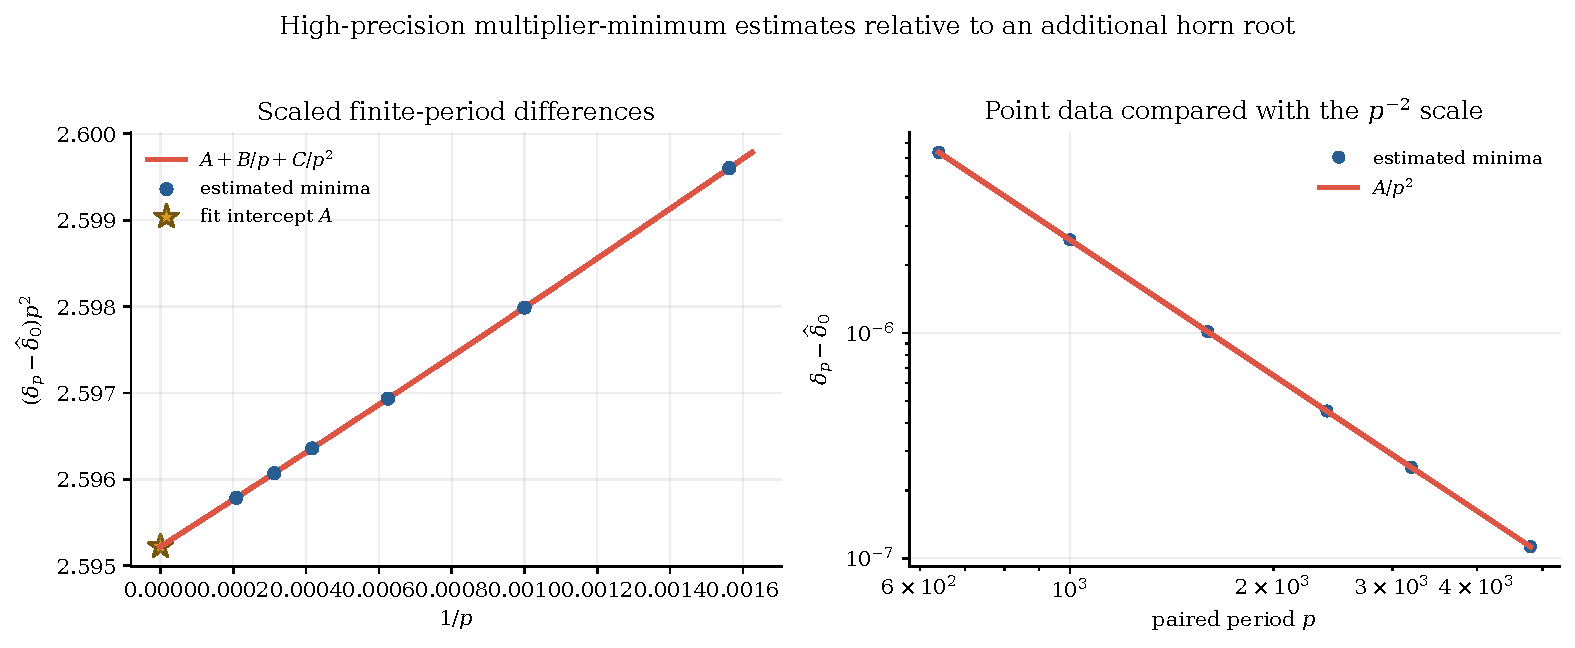
\includegraphics[width=\textwidth]{figures/secondary_rail_convergence.pdf}
  \caption{High-precision multiplier-minimum estimates relative to the midpoint $\widehat\delta_0$ of the certified additional horn-root box.  The empirical fit has intercept approximately $2.59522$; no finite-to-horn identification is inferred from the plot.}
  \label{fig:rail-convergence}
\end{figure}

\section{Local horn reconstruction and asymptotic microscope}

At the additional root, a local reconstructed return centered at
\begin{equation}
  W_0=-12.229425981793852097331\ldots
      -0.140742063517975992036\ldots i
  \label{eq:W0}
\end{equation}
has point jets
\begin{align}
  T'(W_0)&=0.000186514855394184538
           -0.000235537515908513241i,\notag\\
  T''(W_0)&=0.168068815894504543
           +0.133152917422096534i,\notag\\
  T'''(W_0)&=-92.7017750735189+109.473753078838i.
  \label{eq:horn-jets}
\end{align}
Degree-$15$ Cauchy reconstructions at radii $0.004$, $0.005$, and $0.006$ have worst relative discrepancy $6.22\times10^{-18}$.  Chart depths $100$ and $300$ agree through the tested jets to $1.45\times10^{-37}$; deck and half-step covariance residuals are respectively below $4.13\times10^{-53}$ and $1.02\times10^{-46}$.  These are \status{Measured} stability tests around one patch, not directed annular continuation.

The local scale becomes extreme near the fold.  At $\eta=y-y_*=10^{-50}$, the canonical clock predicts a paired period near $3.468\times10^{25}$, and one chamber occupies about $5.767\times10^{-76}$ in the raw $L$ coordinate.  A $1000$-pixel raw-$L$ rendering would therefore require roughly $5.8\times10^{-79}$ per pixel.  Direct orbit rasters at that scale are neither informative nor computationally natural.

The calibrated supplementary microscope instead renders the $E=0$ limiting return in its native cylinder coordinate.  It is an asymptotic template, not a direct $10^{25}$-step orbit computation.  In finite cross-checks, the even limiting core versus direct paired period $640$ has $99.760\%$ strict mask coverage and $100\%$ coarse attraction-class agreement.  The two-dimensional symmetry-reduced odd core versus period $641$ has $91.144\%$ coverage and $99.865\%$ coarse attraction-class agreement, but only its centerline profile is physically calibrated.  Off the centerline, the multiplier-depth discrepancy is large (median $2.2035$ and 95th percentile $8.095$ in $\log_{10}$ units), and three frozen-word mismatches remain in the central core.  The odd off-axis gauge is therefore open.  The full calibration image is retained in the reproducibility supplement because its masks are measured domains, not component boundaries.

\section{What the finite bridge proves---and does not prove}

The intermediate directed work supplies several pieces needed by the hypotheses of \cref{thm:conditional-rail}:
\begin{itemize}[leftmargin=1.5em]
  \item a connected ramified fixed family on $0\le q\le0.00543$, with $y=y_*+q^2$ and directed canonical data;
  \item three parameter slabs in which the same forward orbit tube crosses the attracting tail, core, seam, and outbound region, with combined portal-and-tube weight below $0.11$;
  \item a connected one-step slow-time lemma near the fold;
  \item persistence of the paired period-$640$ phase and its $25/295$ word on a centerline $y$-slab of width $2.2\times10^{-9}$; and
  \item a very strong local quotient defect bound on a tiny $x$-tube over the smallest slab.
\end{itemize}

The strong quotient tube is not attached to the full forward orbit, and the separated slabs have not been joined by one connected relative-gauge enclosure.  Consequently these pieces do not yet prove endpoint matching, cap-to-horn transport, a physical center equation for every large $p$, or component topology.  This is the precise gap between the certified local results and the conditional rail law.

\section{Claim ledger, reproducibility, and next theorem}

\begin{longtable}{@{}>{\raggedright\arraybackslash}p{0.29\textwidth}>{\raggedright\arraybackslash}p{0.13\textwidth}>{\raggedright\arraybackslash}p{0.50\textwidth}@{}}
\caption{Final claim ledger.}\label{tab:claim-ledger}\\
\toprule
Statement & Status & Scope \\
\midrule
\endfirsthead
\toprule
Statement & Status & Scope \\
\midrule
\endhead
Centerline curve and multiplier & \status{Exact} & Baker--Rippon specialization; \cref{thm:fixedcurve}. \\
Dottie identity and quadratic fold & \status{Exact} & Exact identification beyond the prior decimal boundary data; \cref{prop:quadratic-fold}. \\
Two-base family and reciprocal slice & \status{Exact} & \cref{eq:exponential-slice-completion}; $c=1$ and $c=-1$ are sibling slices. \\
Normalized germ and half-step & \status{Exact} & Original $H_y$ is prior; Dottie-normalized \cref{prop:germ} and cylinder lift are used here. \\
Sign-adjusted canonical $E$ and $b$ identities & \status{Exact} & \cref{prop:canonical}; continuation-labelled inverse branches. \\
Horn master, parity, critical-locus, Morse equations & \status{Exact} & Local compatible Fatou continuations; gauge is fixed as stated. \\
Principal/additional even and odd minima & \status{Certified} & One unique root per declared Krawczyk box; no global root count. \\
Periods $639,640,641$ & \status{Certified} & Three local rational windows with cap capture, primitivity, and access stability. \\
Additional finite $640$ witnesses & \status{Certified} & Separate local objects; no common branch or component conclusion. \\
Finite minimum estimates through $p=4800$ & \status{Measured} & Parabolic interpolation, closure, and divisor tests; no stationarity residual or cap marking. \\
Rail asymptotic & \status{Conditional} & Valid under (H1)--(H4) of \cref{thm:conditional-rail}. \\
Full quotient annulus, global root count & \status{Open} & Requires directed overlapping continuation and argument-principle bounds. \\
All-large-period family, topology & \status{Open} & Requires the finite-$E$ cap/gauge/branch matching theorem. \\
Arithmetic or RH implication & \status{Open} & No implication is claimed; no prime indexing, Euler product, functional equation, or positive spectral mechanism is present. \\
\bottomrule
\end{longtable}

The certificates use directed midpoint--radius arithmetic with python-flint 0.9.0 / FLINT 3.6.0 \citep{Johansson2017Arb,FLINT2026}.  Krawczyk inclusions, interval Newton bounds, trapping disks, derivative norms, and divisor exclusions follow the validated-numerics framework of \citet{Krawczyk1969,MooreKearfottCloud2009,Rump2010}.  Every promoted result was replayed at two precisions where the retained record specifies this, with exact rational inputs and outward-rounded output fields.

The reproducibility bundle accompanying this paper contains the frozen phase reports, selected certificate JSON, verification logs, generated figure data, and a SHA-256 manifest.  Four major checkpoint archives have the recorded hashes
\begin{align*}
\text{Phase 3H: }&\texttt{090503b7b958a0cdb1a06d1f8740ea88b8eaadcefcb62c3cbfce3bbe92523dd2},\\
\text{Phase 3J: }&\texttt{3358e50d23ade28b39ffb8ec849aac4dbaecc4521ab8f9b0bd78d98417fc9b7d},\\
\text{Phase 3K: }&\texttt{143e0a82a8d854d09d58206f01c9a5af6e0c44c5b20c36b913a28491f4319f55},\\
\text{Phase 3L: }&\texttt{3c6d2111535c199b1471e0b67b70091d8b45edae4509884f3c8ba76ae007cd6d}.
\end{align*}
The bundle manifest is the controlling inventory; these hashes identify the large frozen checkpoints from which it was assembled.

The next theorem is now narrow and testable: construct a connected chain of directed finite-$E$ Taylor rectangles that attaches the cap-selected forward orbit to the local horn patch, transports the relative Fatou gauge without a branch switch, and preserves the multiplier-Morse equation uniformly.  That theorem would promote one selected rail from \status{Conditional} to \status{Certified}; another raster would not.

\section*{Data and software availability}

All manuscript sources, generated plots, tabulated rail data, claim ledgers, certificate excerpts, and verification instructions are included in the companion reproducibility archive.  The historical full-plane images are retained only as orientation data.  No raw array is inferred from a rendered image, and no certificate is inferred from a pixel color.

\section*{Acknowledgments and disclosure}

The author used AI-assisted symbolic, computational, editorial, and adversarial-audit workflows.  All mathematical claims were re-expressed as exact identities, directed proof objects, finite measured observations, conditional theorems, or open problems before inclusion.  Responsibility for the statements and their interpretation remains with the author.

\bibliographystyle{plainnat}
\bibliography{references}

\end{document}
